\noindent
\graphicspath{{./09-11/Images/}} 
%%%%%%%%%%%%%%%%
% Page de garde
%%%%%%%%%%%%%%%%
\begin{minipage}[t][\textheight][t]{0.33\textwidth}
    \colorbox{StrongBlue}{
        \parbox[c][\textheight][c]{\textwidth}{ 
            \color{OffWhite} 
            \begin{center}
                \noindent
                \begin{minipage}[t][0.55\textheight][c]{0.8\textwidth}
                    {\huge \textbf{Annexe visa marin}}\\

                    \normalsize
                    \begin{center}
                        \begin{tabular}{@{} l @{\hspace{0.5cm}} l @{}}
                            
\includegraphics[width=8px,height=8px]                   {./Pictos/calendar_OffWhite.png} : &\hfill 15-19 Juillet 2026\\
                            &\\
                            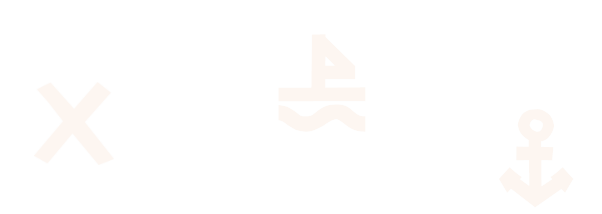
\includegraphics[width=60px,height=20px]                   {./Pictos/trajet_OffWhite.png} \Large  : \normalsize 
                            & \multicolumn{1}{c}{\textbf{Option A}}\\
                            &\hfill Pornic 
\includegraphics[width=8px,height=8px]                   {./Pictos/fleche_OffWhite.png} Pornichet\\
                            &\hfill Pornichet 
\includegraphics[width=8px,height=8px]{./Pictos/fleche_OffWhite.png} La Turballe \\
                            &\hfill La Turballe  
\includegraphics[width=8px,height=8px]{./Pictos/fleche_OffWhite.png} Pornichet \\
                            &\hfill Pornichet 
\includegraphics[width=8px,height=8px]{./Pictos/fleche_OffWhite.png} l'Herbaudière\\
                            &\hfill l'Herbaudière 
\includegraphics[width=8px,height=8px]{./Pictos/fleche_OffWhite.png} Pornic\\
                            &\\
                            
                            & \multicolumn{1}{c}{\textbf{Option B}}\\
                            &\hfill Pornic 
\includegraphics[width=8px,height=8px]                   {./Pictos/fleche_OffWhite.png} l'Herbaudière\\
                            &\hfill l'Herbaudière 
\includegraphics[width=8px,height=8px]{./Pictos/fleche_OffWhite.png} Pornichet\\
                            &\hfill Pornichet 
\includegraphics[width=8px,height=8px]{./Pictos/fleche_OffWhite.png} L’Herbaudière\\
                            &\hfill L’Herbaudière 
\includegraphics[width=8px,height=8px]{./Pictos/fleche_OffWhite.png} Pornic\\
                            &\hfill Pornic 
\includegraphics[width=8px,height=8px]{./Pictos/fleche_OffWhite.png} Pornic\\
                            &\\
                       
                            \makecell{Responsables  \\ de la navigation :}  
                            &\hfill  Aurore Duchemin\\
                            &\hfill  Pierre-Marie Lechevalier\\

                            \makecell{Correspondants \\ à terre :}  
                            &\hfill  Théo Le Dru\\
                            &\hfill  Pierre-Olivier Greil \\

                            &\\
                            Staff navigation : &\hfill\\
                                        &\hfill Aurore Duchemin (CF)\\
                                        &\hfill Pierre-Marie Lechevalier (CF)\\
                                        &\hfill Camille Trefoux (PE)\\
                                        &\hfill Mathis Bernard-Dumas (PE)\\
                                        &\hfill Eliott Bourlon (PE)\\
                                        &\hfill Raphaël Monet-Stopp (PE)\\
                                        &\hfill Jules Hilling (PE)\\
                                        &\hfill Yoann (PE)\\
                                        &\hfill Bapiste Gutton(PE -16 ans)\\
                                        &\hfill Julie Menard(PE)\\
                            \end{tabular}
                    \end{center}
                     
                \end{minipage}%
            \end{center}       
        }      
    }
\end{minipage}%
\begin{minipage}[c][\textheight][t]{0.1\textwidth}
\hfill
\end{minipage}%
\begin{minipage}[c][\textheight][t]{0.50\textwidth}
    \vspace{1.5cm}
    \color{StrongBlue}    
        {\huge \textbf{Description du projet}}\\
      
        \vspace{1cm}
        {\huge \textbf{Description de l'unité et du staff nautique}}\\
            L'unité est composée de x jeunes. Les pionniers caravelles marines d'Irigny ont leurs premiers PE depuis l'été dernier, le groupe à récemment ouvert une branche marine. C'est son premier camp embarqué. L'unité à en revanche l'habitude de naviguer à la fois sur des habitables en plan d'eau intérieurs mais aussi en Méditérranée. 
            
            \vspace{1cm}
            { \huge \textbf{Supports}}\\
            La flotte est composée de sept bateaux dont la répartition est la suivante : \\
            Quatre Kelt 620 : \textit{Dream}, \textit{Morvan}, \textit{Douce} et \textit{Doudou} \\
            \makebox[\textwidth][c]{
                \textbullet \hspace{0.2cm} Longueur : 6.20 m, \hspace{0.3cm} 
                \textbullet \hspace{0.2cm} largeur : 2.50 m, \hspace{0.3cm} 
                \textbullet \hspace{0.2cm} tirant d'eau : 1.20 m, \hspace{0.3cm}    
                \textbullet \hspace{0.2cm} couchages : 4
            }\vspace{0.1cm}\\
            Un Jeanneau Rush : \textit{Maurice} \\
            \makebox[\textwidth][c]{
                \textbullet \hspace{0.2cm} Longueur : 9.50 m, \hspace{0.3cm} 
                \textbullet \hspace{0.2cm} largeur : 3.15 m, \hspace{0.3cm} 
                \textbullet \hspace{0.2cm} tirant d'eau : 1.40 m, \hspace{0.3cm}    
                \textbullet \hspace{0.2cm} couchages : 6
            }\vspace{0.1cm}\\
            Un Feeling 306 Di : \textit{Kirie} \\
            \makebox[\textwidth][c]{
                \textbullet \hspace{0.2cm} Longueur : 9.02 m, \hspace{0.3cm} 
                \textbullet \hspace{0.2cm} Largeur : 3.15 m, \hspace{0.3cm} 
                \textbullet \hspace{0.2cm} tirant d'eau : 0.70 m, \hspace{0.3cm}    
                \textbullet \hspace{0.2cm} couchages : 6
            }\vspace{0.1cm}\\
            Un Oceanis Clipper 311 : \textit{Avel} \\
            \makebox[\textwidth][c]{
                \textbullet \hspace{0.2cm} Longueur : 9.85 m, \hspace{0.3cm} 
                \textbullet \hspace{0.2cm} Largeur : 3.50 m, \hspace{0.3cm} 
                \textbullet \hspace{0.2cm} tirant d'eau : 1.45 m, \hspace{0.3cm}    
                \textbullet \hspace{0.2cm} couchages : 5
            }\\
            \vspace{0.5cm}
            La flotte devant être coupée en deux flotilles pour des raisons réglementaire, les kelts, supposés moins rapide, seront regroupés dans la même flotille. Les trois autres bateaux plus homogènes seront regroupés ensemble. \\
            L'objectif est que les départs et arrivés aux ports soient groupés mais que chaque flotte puisse évoluer à son rythme une fois en mer.\\
            Il est envisagé de mixer les flotilles dans le cas ou certains des kelts nécessiteraient des remorquages, cas dans lequel les kelts seraient séparés en deux groupes.  
\end{minipage}%
%%%%%%%%%%%%%%%%
% Page de Gauche
%%%%%%%%%%%%%%%%

\begin{minipage}[t][\textheight][t]{0.33\textwidth}
    \colorbox{StrongBlue}{
        \parbox[c][\textheight][c]{\textwidth}{ 
            \color{OffWhite} 
            \begin{center}
                \noindent
                \begin{minipage}[t][0.85\textheight][c]{0.8\textwidth}
                    \normalsize
                    
\begin{center}
{\huge \textbf{Journée type}}\\ \vspace{0.5em}

\renewcommand{\arraystretch}{1.40}
\begin{tabular}{|C{3em}|C{12em}|}
\hline
\textbf{Heure} & \textbf{Activité} \\
\hline
7h30  & Réveil, petit déjeuner et mise en condition de navigation des bateaux \\
\hline
8h30  & Brief de navigation + conseil de flotille \\
\hline
9h00  & Appareillage, encas en navigation \\
\hline
12h30 & Déjeuner et repos \\
\hline
14h00 & Deuxième partie de navigation, goûter en mer \\
\hline
17h00 & Arrivée au port, amarage \\
\hline
17h30 & Débriefing de navigation \\
\hline
18h00 & Douche et préparation du repas \\
\hline
19h00 & Repas \\
\hline
20h30 & Veillée. En cas de mouillage, la veillée est avancée à 20h et la vaisselle est faite au retour de la veillée. \\
\hline
22h00 & Chaque jeune est dans son bateau \\
\hline
22h30 & Silence sur le camp \\
\hline
\end{tabular}
\end{center}

\vspace{1cm}
La journée type dimensionne la durée des navigations. 
Elle a néanmoins vocation à être ajustée lors des nuits au mouillage, permettant ainsi de descendre à terre pour les veillées, tout en étant de retour aux bateaux avant le coucher du soleil.
Les équipages de navigation sont autant que possible mixtes afin de varier les découvertes et d'homogénéiser les niveaux de navigation. 
Les deux navigations de sortie de mouillage se feront toutefois en équipe de vie. 

                \end{minipage}
            \end{center}       
        }      
    }
\end{minipage}%
\begin{minipage}[c][\textheight][t]{0.10\textwidth}
\hfill
\end{minipage}%
\begin{minipage}[c][\textheight][t]{0.50\textwidth}
    \vspace{1cm}
    \color{StrongBlue}    
        % TODO
        {\huge \textbf{Description de l'itinéraire}}\\
        \begin{figure}[H]
            \centering
            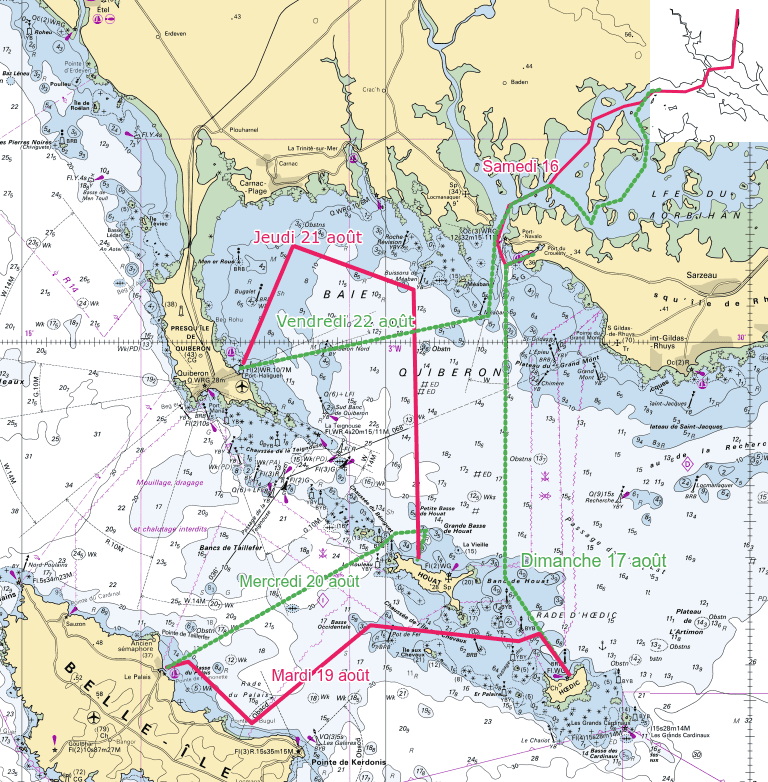
\includegraphics[height=0.5\textheight]{Templates/carte_globale.png}
        \end{figure}
    
        Les trajets quotidiens ne sont pas trop long et laissent du temps pour jouer sur l'eau. Ce temps de jeu est souvent positionné vers la fin de la navigation, il pourra être utilisé pour se diriger vers un abris de replis si celui escompté est plein. 

        Enfin, et car même en août la météo bretonne est susceptible d'être capricieuse, une étape peut être supprimée soit à Houat soit à Port Haliguen sans compromettre le reste de la navigation si un jour de retard est pris sur le planning initial. 
     
        {\vspace{1cm}\huge \textbf{Plan d'eau : baie de quiberon}}\\
            Les courants dûs aux marées jouent un rôle important dans toute la zone de navigation, particulièrement à proximité de l’entrée du golfe. L'amplitude de ces effets évoluera en fonction des coefficients de marée qui seront compris entre 44 et 87 pour la durée de l'itinérance. 
            Les secteurs de vents dominants sont principalemment Ouests sur la période estivale. 
            Enfin la présence des différentes Îles (\textit{Belle Île}, \textit{Hoëdic}, \textit{Houat}) et de la presqu'île de \textit{Quiberon} permettent de casser la houle ne laissant virtuellement que les effets de la mer du vent.      

\end{minipage}%

       



%%%%%%%%%%%%%%%%
% Page de droite
%%%%%%%%%%%%%%%%
\newgeometry{top=1cm, bottom=2cm, left=1cm, right=1cm}
\begin{minipage}[c][0.9\textheight][t]{\textwidth}
    \color{StrongBlue}    
    \noindent
    \centering 
    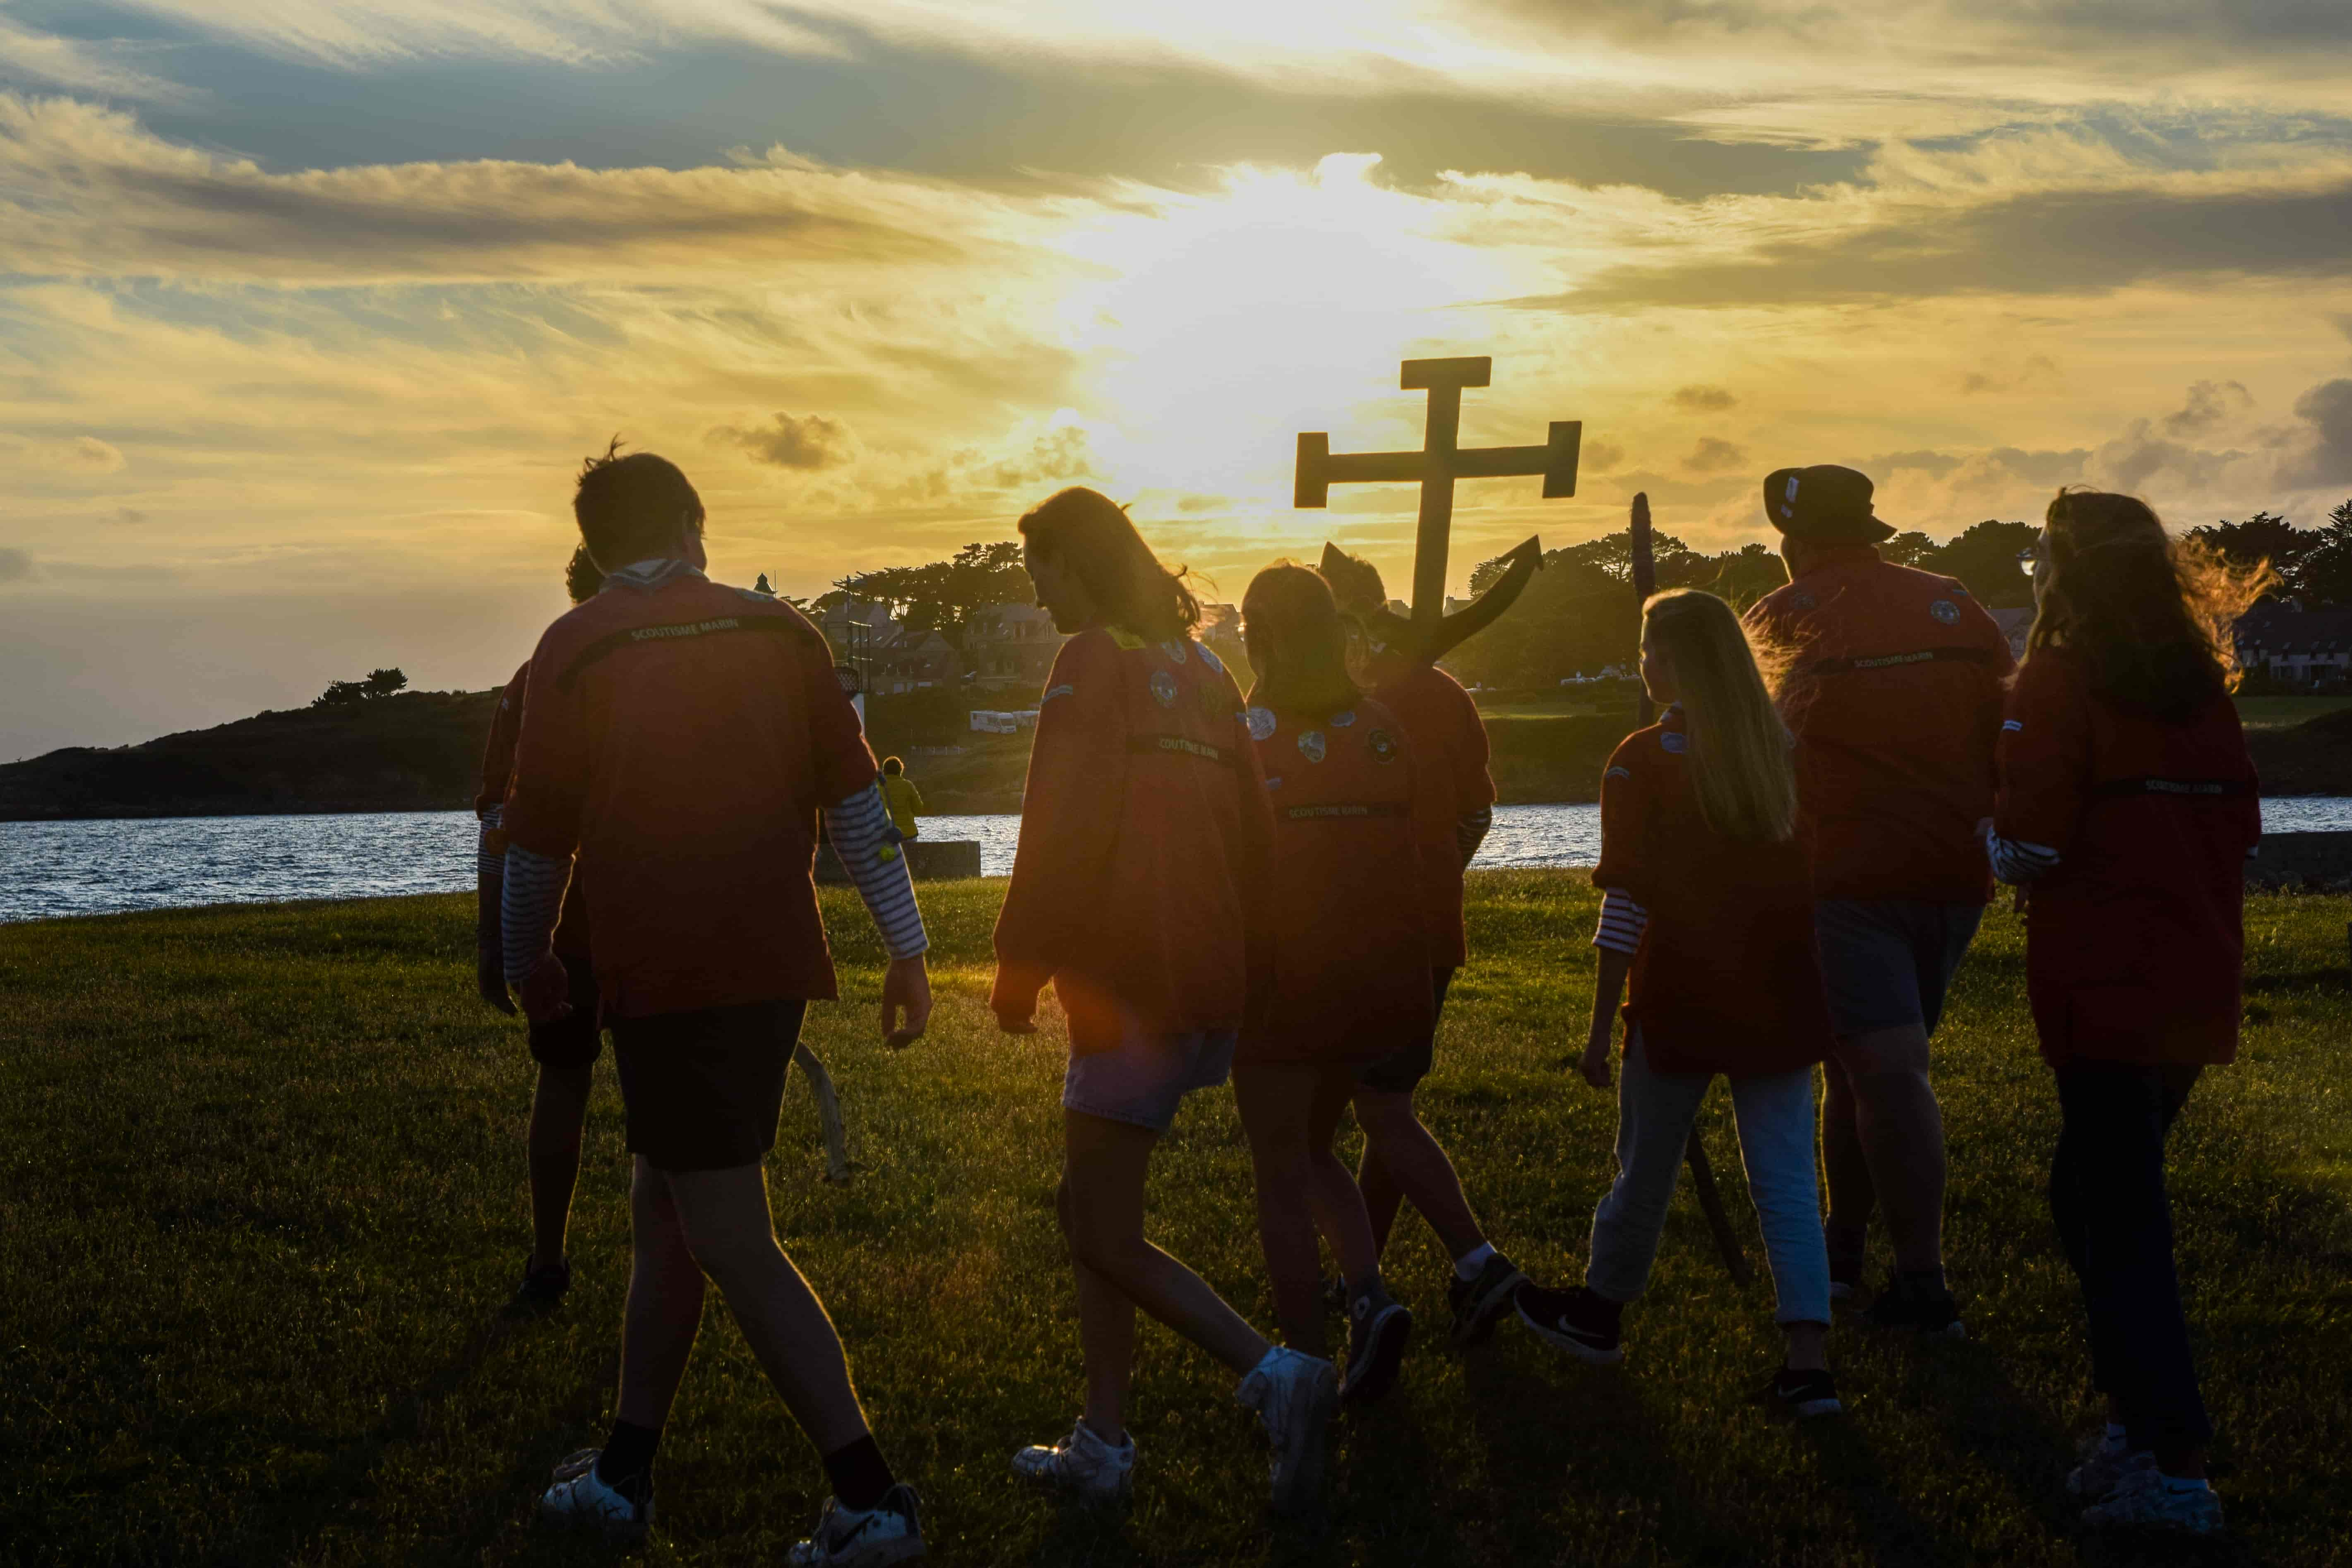
\includegraphics[height=\textheight, width=\textwidth, keepaspectratio]{Templates/horizontal.jpg}
\end{minipage}%
\restoregeometry



